\section{Results}\label{sec:results}


\subsection{Proposition 1: Increasing cross-organisational transparency of information is a necessary condition for cross-organisational CI\&D.}

{\bf .}

\subsection{Proposition 2: Increased cross-organisational transparency of information is considered positive.}

Increasing cross-organisational transparency can be perceived differently by different stakeholders. The interviewees were asked how they considered the increase of transparency across companies, and how they perceived business and personal relationships between companies. The complexity of the project is experienced as an impediment working against full transparency of information.

However, the interview results support the proposition, and the increase of information transparency is generally considered positive. This answer to proposition 2 is deduced from the following findings:

\noindent {\bf F2.1: Increased transparency is positive.} All the interviewees experience positively the increase of cross-organisational transparency between companies and employees, for both business and personal relationships between companies. The interviewees experience positive effects in terms of more awareness of the project status and increased mutual understanding. In particular, Volvo employees found sharing a workplace with Delphi developers especially effective for creating a shared mental model, thanks to the closer interaction with e.g. software developers.

\noindent {\bf F2.2: Trust is increased.} The increase of transparency of information increases trust, too, on two levels. Firstly, increased trust between stakeholders improves collaboration and communication. Secondly, the trust gained in past project (thanks to increased transparency of information) is more easily adopted in future projects as well. 

\subsection{Proposition 3: Cross-organisational sharing of information is considered simple between members of the projects.}

This proposition challenges the interviewees to critically evaluate the level of difficulty to share information across companies. In particular, the interviewees were asked about the difficulty to share information and the role of physical distance. The VCC/Delphi project is perceived as a complex project by both companies. Due to the complexity of this project, the project members experience that it is difficult to work against full transparency of information with other stakeholders. It is extremely difficult in the automotive industry to manage responsibilities on hardware and software (responsibility split) and managing intellectual property (IPR).

The findings partially support the proposition. The tooling and cross-organisational transparency, for example reducing physical distance, benefit cross-organisational information sharing, hence, reducing the complexity of a project. However, the automotive industry experience difficulty to share information, and manage responsibilities and IPR. This answer to proposition 3 is deduced from the following findings:

\noindent {\bf F3.1: Reducing physical distance most efficient.} The interviewees argued that reducing the physical distance between project members is the best situation for information sharing. The new way of working introduced in the VCC/Delphi project better enables the developers, but also management staff, to share information more efficient.

\noindent {\bf F3.2: Tooling support information sharing.} The tooling used for sharing information between developers or management staff is also a crucial factor for efficient information sharing across, but also within, companies. The interviewees from the VCC/Delphi project are positive about the tools and their supportive role in the project and agree that it reduces the complexity of the project.

\noindent {\bf F3.3: Managing responsibilities and IPR.} \pat{Add something about managing responsibilities and IPR}

\subsection{Proposition 4: Project members have sufficient information to perform their activities.}

This proposition challenges the interviewees to critically evaluate information, sent and received, between project members. They were asked what kind of information is (not) shared, if they have sufficient information available to perform their activities, and how this compares to other projects. All technical information is shared between project members, this includes source code, project information, and time planning. Commercial information is not shared between project members. This information contains strategic decisions, estimations, and third party agreements. The increased transparency across companies result in much more information than traditional projects, but equal or a bit more than agile projects. Third party agreements are an impediment for full transparency, because of licensing and responsibility issues.

However, the findings support this proposition and prove that project members have sufficient information available for their activities. This answer to proposition 4 is deduced from the following findings:

\noindent {\bf F4.1: Project members have sufficient information.} Both companies, VCC and Delphi, state that they have sufficient information available from both companies to perform their activities. 

\noindent {\bf F4.2: Lack overview in overall project.} The interviewees expressed that they miss an overview of their contribution in the product and overall project. Volvo hosted a presentation about the RFQ process and project details. This was perceived as positive by Delphi.


\subsection{Proposition 5: A more open transparency policy improves the quality of the project and its results.}

This proposition is developed to investigate whether the quality of the project results benefit from a more open transparency policy across companies. During the interview survey, the interviewees were asked a question about the effects of this policy on the project and its results. 

Findings emerging from the interviews are:

\noindent {\bf F5.1: High level of Quality.} The interviewees were unanimous about the positive effects on the quality of the project and its results. The quality improvements are already visible in the early stage of the project and they are confident about the improvements in the long term. An open transparency policy is positive for quality control because of mutual understanding of the project status and as a result, gaining efficiency. Delphi experiences healthy pressure on their activities and forces them to a certain quality level, because the customer is involved in the process of the product. To preserve the quality of the progress, Volvo is not heavily involved in the process.


Accordingly, we elicit the following possible answer to proposition 5:
The findings support this proposition and prove the quality of the project and its results improve due to a more open transparency policy across companies.

\subsection{Proposition 6: Strict contract-based collaboration is an impediment for cross-organisational Continuous Integration and Deployment}

This proposition challenges how practitioners experience a strict (or closed) contract in a cross-organisational setting where companies work together in software engineering projects using Continuous Integration and Deployment (CI\&D). During the interview survey, the interviewees were asked questions on the role of the contract when looking at information sharing and cross-organisational CI\&D. During the research it became clear that information sharing is seen as a crucial factor for cross-organisational collaboration. A closed contract regulates traditional project setups where the customer defines a list of requirements and the supplier has to fulfil it within a given time frame and budget. Originally the automotive industry is traditional and relatively closed. It however emerges that it changing towards greater cross-organisational transparency, participation in open source projects, and becoming a software-intensive sector. While still ongoing, this transition is confirmed by all interviewed stakeholders, and could lead to a cultural change toward adopting more open or agile contracts for cross-organisational CI\&D.

\begin{figure}[htb]
\centering
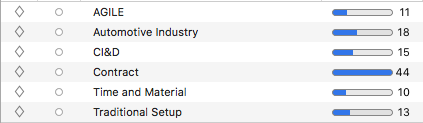
\includegraphics[width=\columnwidth]{figure/ss_CodeGroup6.png}
\caption{Cultural change toward adopting more open or agile contracts for cross-organisational CI\&D}
\label{fig:towardsAgile}
\end{figure}


Findings emerging from the interviews are:

\noindent {\bf F6.1: Agile contracts favour cross-organisational collaboration.} The interviewees share the opinion that a more open (or agile) contract would be healthier for the project and benefit cross-organisational collaboration. Although some of the project members from both customer and supplier companies are not fully aware of the contract details, they do share the feeling of being restricted. They believe that strict contracts conflict with an agile way of working instead of supporting it, and suggest to adopt more agile contracts, instead, also referred to as Time and Materials (T\&M) contracts\footnote{According to a T\&M contract, the contractor is being billed per hour regardless of the software project duration. If any additional features have to be developed the supplier charges just for the time spent by its employees working on a certain set of tasks [en.wikipedia.org]. This brings high flexibility to accommodate projects with evolving requirements, but also high uncertainty about the related costs.}. 
The interviewees agree that a T\&M contract allows for a better adaptation to project changes, distribution of resources, and it creates shared ownership otherwise hindered by closed contracts. They also argue in favour of a combination of a fixed price and T\&M contract, where stakeholders would agree on the product and cost estimation, but maintain high flexibility on how to produce it. This combination fulfils the need for flexibility and agility, but also the security for the customer. All interviewees made it clear that good collaboration between their companies is important from a legal and contractual perspective to support cross-organisational CI\&D.

\noindent {\bf F6.2: Closed contracts ease negotiation.} For a customer it is (still) more comfortable to work with closed contracts because one has more leverage and binds the supplier to pre-defined deliverables and deadlines. A Volvo manager involved in a RFQ projects, further states that it is hard for suppliers to negotiate with a T\&M or other agile contracts, and that closed contracts make it easier competing with other suppliers.

Accordingly, we elicit the following possible answers to proposition 6:

\begin{itemize}
\item Cross-organisational CI\&D benefits from a more open collaboration among companies, such as information sharing and adaptation to project changes. A strict contract is an impediment for this way of working related to cross-organisational CI\&D.
\item A strict contract is an impediment for cross-organisational CI\&D. Although there is no direct connection between a strict contract and cross-organisational CI\&D, the way of working related to this method benefits from an open or agile contract.
\item Cross-organisational CI\&D is possible with a strict contract, but synergy effects, i.e. collaboration and flexibility, are in effect when supported by an agile contract. By taking the synergy effects into account, a strict contract can be an impediment for Cross-Organisational CI\&D. An agile contract is difficult for a RFQ due to the open and uncertain characteristics of the contract.
\end{itemize}

\subsection{Proposition 7: If information is precise then, even though information is exchanged frequently, information overload is unlikely to be considered a problem.}

The assumption was that because of increased transparency between companies, information overload could occur. This proposition was developed to challenge project members how they experience information sharing. The interviewees were asked what kind of information is (not) shared, if it is much more or less information than other projects, and if they experienced information overload in their situation. Information precision is information sharing where supply and demand of information is synchronised. Information overload is information sharing where the receiving organisation receives more information than necessary. All the interviewees argued that information overload was not seen as a problem or risk.

Findings emerging from the interviews are:

\noindent {\bf F7.1: Understanding due collaboration.} 

\begin{itemize}
\item It is important to have an understanding, as result of clear collaboration and communication, of information needed by the receiving stakeholder, this prevents overreaction.
\item It is important to have an understanding of information needed by the receiving stakeholder, this prevents overreaction. This is achieved by clear collaboration and communication on what is necessary to share.
\end{itemize}

Accordingly, we elicit the following possible answer to proposition 7:

The findings support the proportion and information overload is not experienced as problem.



\subsection{Proposition 8: Standards and processes, based on industry-wide data and process standards benefit cross-organisational CI\&D.}

This proposition challenges the interviewees to experience the effects of industry-wide standards and processes in a cross-organisational setting where companies work together in software engineering projects using Continuous Integration and Deployment. The interviewees were asked if they use industry-wise standards or open source projects, and whether they find them beneficial for information sharing, which is important for cross-organisational CI\&D. The automotive industry is participating in more open source projects (i.e. AUTOSAR and GENIVI) and attempt to be good open source citizens. This development allows companies to hire new employees easier, because open source knowledge is more common than knowledge of proprietary technology.

Findings emerging from the interviews are:

%\begin{itemize}
%\item 
\noindent {\bf F8.1: Beneficial for information sharing.} The industry standards and open source projects allow a common language (i.e. AUTOSAR framework) and shared knowledge between project members, which makes it easier to communicate and share information.
%\item 

\noindent {\bf F8.2: Maturity and Management.} It is important for the success and adoption of open source projects and standards, that they are highly controlled by one person or organisation. According to several interviewees, the maturity is the crucial factor for the success or failure of an industry standard or open source project.
%\end{itemize}

Accordingly, we elicit the following possible answer to proposition 8:

Industry standards and open source projects allow a common language and shared knowledge, therefore, benefits information sharing, which is important for cross-organisational CI\&D.






% {\bf Industry Perspective.} 
% To preserve an open approach to the project, a product manager at a software development company suggests a combination of an agile and fixed price contract by creating project branches to avoid overhead in the main project.
%
%(Y)
% {\bf Maturity.} The automotive software ecosystem needs to adapt to the needs from the stakeholders. The industry is not mature enough, but is improving to adopt cross-organisational Continuous Integration and Deployment.
% Yes: Johnny Karlsson, Darrel Cullen, Lars Mattson, Petter Molder, Jacob Juul, Matti Larborn, 
% No: Anders Lindbom, Michael Svenstam, Mattias Almljum